\documentclass[a4, 11pt]{article}
\usepackage{hyperref}
\usepackage[table,xcdraw]{xcolor}
\usepackage{pgfgantt}
\usepackage{geometry}

 \geometry{
 a4paper,
 left=1in,
 right=1in, 
 top=1.44in,
 bottom=1.44in
 }

\usepackage[english]{babel}
\usepackage[utf8]{inputenc}
\usepackage{csquotes}
\usepackage{graphicx}
\usepackage{subfig}
\usepackage{fancyhdr}
\usepackage{lscape}
\usepackage{enumitem}
\usepackage{fancyvrb}

\pagestyle{fancy}
\fancyhf{}
\lhead{Uppsala University}
\setlength{\headheight}{20pt}
\cfoot{\thepage}
\rfoot{Financial Streams}
\renewcommand{\headrulewidth}{0.5pt}
\renewcommand{\footrulewidth}{0.5pt}

\usepackage[backend=biber,sorting=none]{biblatex}
\addbibresource{sources.bib}



%%%%%%%%%%  LOCAL VARIABLES HERE
\newcommand{\thesistitle}{Bivariate Trend Calculus and Causal Inference on Financial Streams}
\newcommand{\LIF}{}
\newcommand{\sdml}{ScaDaMaLe}
\newcommand{\quotes}[1]{``#1''}
\newcommand\tab[1][1cm]{\hspace*{#1}}



\begin{document}
\begin{titlepage}

\begin{figure}
   \vspace{0.2in}
   \begin{center}
     
\includegraphics[scale=0.5]{Images/UU_LOGO.png}
   \end{center}
\end{figure}

\thispagestyle{fancy}

\vspace{1in}

\center

\textsc{\large Project in Data Science }

\vspace{0.6in}

\noindent\vspace{0.1in}\makebox[\linewidth]{\rule{\linewidth}{1.2pt}}
\textsc{ \textbf{\large \thesistitle{}}}
\noindent\makebox[\linewidth]{\rule{\linewidth}{1.2pt}}

\vspace{0.5in}

 \begin{minipage}{0.58\textwidth}
    \begin{flushleft}
        \textit{Students:} \\
        Stavroula Rafailia Vlachou \\
        Virginia Jimenez Mohedano\\
        stavroula.vlachou.2231@student.uu.se\\
         virginia.jimenezmohedano.6097@student.uu.se
    \end{flushleft}
 \end{minipage}
\begin{minipage}{0.38\textwidth}
    \begin{flushright}
    \textit{Supervisor:} \\
    Raazesh Sainudiin \\
    raazesh.sainudiin@math.uu.se
    \end{flushright}
\end{minipage}

\vspace{1.6in}

\textbf{\large Department of Information Technology} \\

\today

\end{titlepage}


\newpage
\begin{abstract}
    Analysing time series and identifying trends can become quite computationally heavy, especially in cases that include big data that needs to be processed on real time. This paper presents a computationally efficient solution for long term trend finding on bi-variate financial time series, by integrating the TrendCalculus library within the Apache Spark ecosystem. An extension is also implemented as an attempt to find causal inference among the established trend change points. The latter is achieved by utilising the Pathogen algorithm. 
    
\end{abstract}
\begin{center}
    \textbf{Keywords:} Financial time series, long term trends, causal inference, 
\end{center}
\setcounter{page}{2}
\newpage


\tableofcontents
\newpage


\section{Introduction}
This project amounts to identifying long term trends on time series from historical data and is an attempt towards performing a scalable data science pipeline for causal inference on trend change events of high order. Although the analysis is focused on financial time series, any time series of interest can be used as an input. 


\section{Approach}
For the analysis the following tools and frameworks were utilised:
    \begin{enumerate}
        \item Historical data of financial time series \cite{HistData}.
        \item The Apache Spark ecosystem \cite{Spark} to handle the big volume of the data. 
        \item The TrendCalculus algorithm \cite{TrendCalculus}, which provided an efficient solution on identifying long term trends by establishing high order trend change points.
        \item The Pathogen algorithm \cite{Pathogen} to establish causal inference between events of two time series. 
    \end{enumerate}
    


\section{Methods}
\subsection{The pipeline}
Figure \ref{fig:pipeline} presents the main steps of the overall application.  
\vspace{0.2in}
\begin{figure}[!ht]
    \centering
    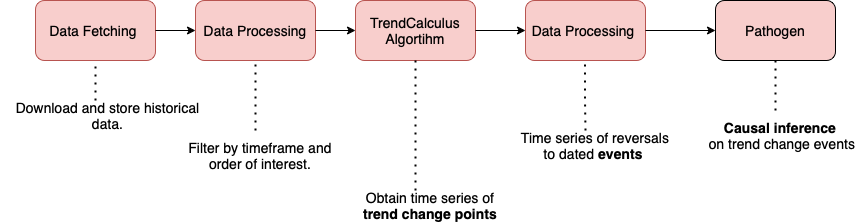
\includegraphics[width=1\textwidth]{Images/Pipeline.png}
    \caption{Summary of the main steps of the pipeline}
    \label{fig:pipeline}
\end{figure}
 
  %\textsf{\textbf{Causal inference:}} The returned time series was encoded to be suitable as input to Pathogen by turning consecutive  $n$-th order reversals to events.\\
 
\subsection{The data}
In this work we utilised historical data from the foreign exchange market \cite{Forex} for the trading of currencies. The data sets consist of $66$ pairs of currencies and futures/commodities with values recorded every one minute over the last two decades. The obtained data were fetched from \cite{HistData}, structured as comma separated values (.CSV format). Each financial time series is associated with a ticker which is used in order to download all the files associated with the desired trading pair. This ticker is then used to combine all of the available data files into a single one using methods from \cite{FX1}. The latter is then written as parquet files on Databricks file system (dbfs). This way each financial time series is uniquely identified given the ticker name associated with it and all of the relevant records can be loaded at once. 

\subsection{Cloud Computing}
A cluster was deployed in order to distribute the computational tasks and scale on demand within the Apache Spark framework. To handle the big volume of the data that are to be processed and execute the computations within a reasonable time frame, the Apache Spark ecosystem and it's tools are put into action. Specifically, a Spark cluster was deployed so that the application can be scalable not only in terms of I/O but also in computing power when necessary. This way, the distribution of computational tasks is enabled and the application can scale on demand.  In addition, after the most computationally intensive levels of the pipeline the processed data are written as parquet files on the Databricks file system (dbfs). At the same time, throughout the process several checkpoints are kept to avoid exploding computations of complex queries.

% In addition, the algorithm of choice for the establishment of long term trends provides an efficient solution to the problem, since on every iteration there is a significant data reduction while losing no information. \\
%To finalise, Pathogen algorithm is utilised in order to establish casual inference between events from the two time series.

\subsection{The TrendCalculus algorithm}
In order to establish long term trends on time series we implemented the TrendCalculus algorithm and focused the analysis on data from the financial sector. This section gives an overview of the algorithm and the necessary processing that was implemented in several stages of the pipeline. 

\subsubsection{Definitions}
\textbf{Rising trend}: a trend is defined as rising if it has higher Highs and higher Lows.\\
\textbf{Falling trend}: a trend is defined as falling if it has lower Highs and lower Lows.\\[2ex]
The above definitions can be quantified by assigning the values of $+1$ for rising trends and $-1$ for falling trends. Figure \ref{fig:RisingAndFalling} illustrates two examples of the above definitions. 
\begin{figure}[!ht]
    \centering
    \subfloat[\centering Rising Trend]{{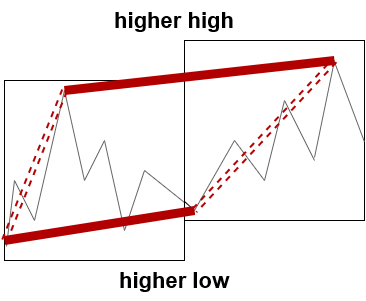
\includegraphics[width=6cm]{Images/RisingTrend.png} }}%
    \qquad
    \subfloat[\centering Falling Trend]{{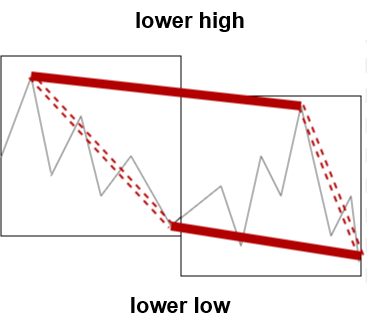
\includegraphics[width=6cm]{Images/FallingTrend.png} }}%
    \caption{Example of a rising trend on the left and a falling trend on the right}%
    \label{fig:RisingAndFalling}
\end{figure}

\subsubsection{The algorithm}
The TrendCalculus algorithms implements the following steps iteratively:
\begin{itemize}
    \item Stream the data across a fixed window size. 
    \item For each window identify the dated High and Low. 
    \item Summarise each window as rising or falling (based on the order of occurrence of the Low/High; a window is characterised as rising if the Low is followed by the High and falling for the opposite case).
    \item Compare the summary of the current window to the previous one. 
    \item Assign a sign for each window according to the TrendCalculus equation \ref{TrendCalculusEquation}. 
\end{itemize}
\begin{equation}\label{TrendCalculusEquation}
    sign(sign(H_{p_i}-H_{p_{i-1}})+sign(L_{p_i}-L_{p_{i-1}}))
\end{equation} where 
\begin{itemize}
    \item H, L $=$ High, Low 
    \item $p_i=$ current window
    \item $p_{i-1}=$ previous window
\end{itemize}
\textbf{Reversal point:} A point on the previous window where the trend values flip.\\[2ex]
\textbf{Reversal Finding Rule:}
\begin{itemize}
    \item If the trend moves from $+1$ to $-1$ (from rising trend to falling) then the previous high is a reversal point.
    \item If the trend moves from $-1$ to $+1$ (from falling trend to rising) then the previous low is a reversal point. 
\end{itemize}

\textbf{The FHLS data structure:}\\
By looking at the last step of the TrendCalculus algorithm one notices that the outcome of a window's summary may be $0$, according to equation \ref{TrendCalculusEquation}. To handle this special case, the following data structure is introduced. \\
\textbf{F}: First of H/L\\
\textbf{H}: High\\
\textbf{L}: Low\\
\textbf{S}: Second of H/L\\[2ex]
The above data structure is used to provide an additional summary on zero-windows by using the Second H/L of the previous window and the First H/L of the current window. This additional-intermediate window is then used as a regular window to find the trends after comparison with the previous and current window. Lastly, the reversals are then found as usual since all of the windows are now either rising or falling and the reversal finding rules can be applied. \\[2ex]
The output of the above algorithm is a time series of reversal points or in other words a time series of trend change points. The returned time series can be used as input to the algorithm iteratively in order to find reversals of higher order and establish long term trends. What is worth mentioning is that by doing so, no information is lost since a reversal of order $n$ is also a reversal of order $n-1$. This stacking of TrendCalculus time series provides an efficient solution on finding high order reversals, since on each iteration performed, the data is reduced until no points are available or the required number of points are summarised (all reversals of a given order have been established). 


\section{Results - Showcases}
For illustration purposes two pairs of time series are put into production and the outputs of the TrendCalculus algorithm are plotted on the same graph. The chosen records concern the Gold ounce in USD against the Oil price and the stock market in the same currency. For the Oil price the Brent Crude Oil time series is used, as it is one of the types of crude that plays a key role on setting the oil price on the market. As a representative of the stock market the Standard $\&$ Poor $500$ index (S$\&$P$500$) was chosen. 


\subsection{Gold ounce in USD Vs. Brent Crude Oil Price in USD}
For this first showcase the financial time series used are Gold ounce and Brent Crude Oil price in USD; a pair often considered as the main representative of large commodity markets. From a trading point of view gold has been the most effective safe haven in most countries and is usually seen as a hedge against inflation by investors. At the same time, according to Research published in 2017 in the journal Economic Research \cite{EconomicJournal} increasing oil prices can lead to inflation. Naturally, the question that rises is:
\begin{center}
    \textit{Can a change in oil price can be a predictor of a change in gold price?}\\[2ex]
\end{center}
\begin{center}
\textit{Over the long term gold prices tend to move up and down in tandem with oil prices} \cite{OilPrice}.    
\end{center}
As can be seen in Figure \ref{fig:GoldOilScalled}, this long term co-movement is indeed verified for the last two decades.
\begin{figure}[!ht]
    \centering
    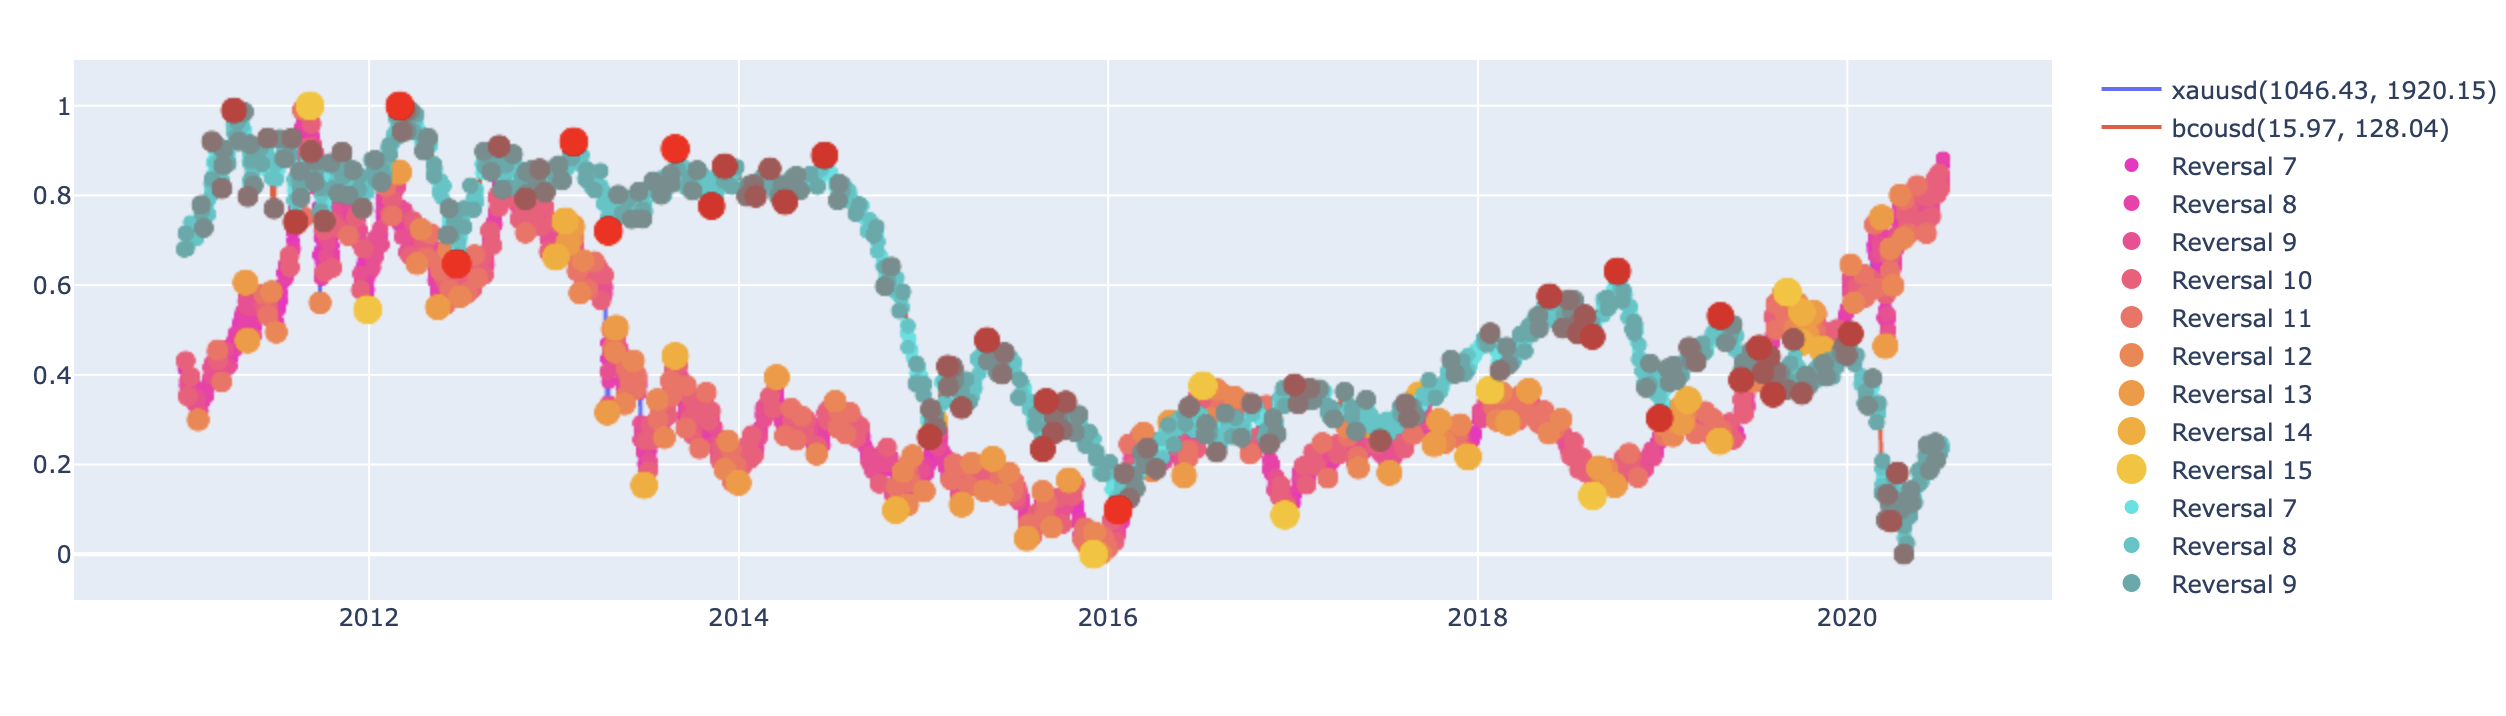
\includegraphics[width=1.1\textwidth]{Images/GoldOil.png}
    \caption{Gold ounce in USD vs Brent Crude Oil in USD (scaled)}
    \label{fig:GoldOilScalled}
\end{figure}

\subsection{Gold ounce in USD Vs S\&P500 index}
For the second showcase the gold price is compared against the S$\&$P$500$ index. The latter is a stock market index tracking the performance of $500$ large companies across all industries in the United States. It includes both growth stocks and values stocks and it is often considered to be one of the best representations of the U.S. stock market. Generally, the dominant intuition within the financial sector regarding the relation between the two stocks is the following: 
\begin{itemize}
    \item Stocks tend to benefit from economic growth and stability.
    \item Gold rises in times of economic distress and crises.
\end{itemize}
This intuition is further confirmed by historical data that usually show that gold performs better than stocks in times of market downturn. In order to give an example of this long term inverse movement we focus on the events after the stock market crash of February $2018$.\\[2ex]
On Monday the $5^{th}$ of February $2018$, an event often characterised as “Volmageddon” (Volume Armageddon), the $S\&P500$ index saw one of the largest one-day point drop in history by $113.19$ points. Despite the fall of the rest of the stock market indexes that followed, gold improved. During the first few months after Volmageddon both commodities fluctuated without any major ups or downs. However, from May of the same year S$\&$P$500$ started to steadily grow, while gold plunged hitting a significant low on August. The graph of Figure \ref{fig:GoldSP500Scalled} illustrates the two time series over the year $2018$, where the previously described inverse movement can be clearly observed. 
\begin{figure}[!ht]
    \centering
    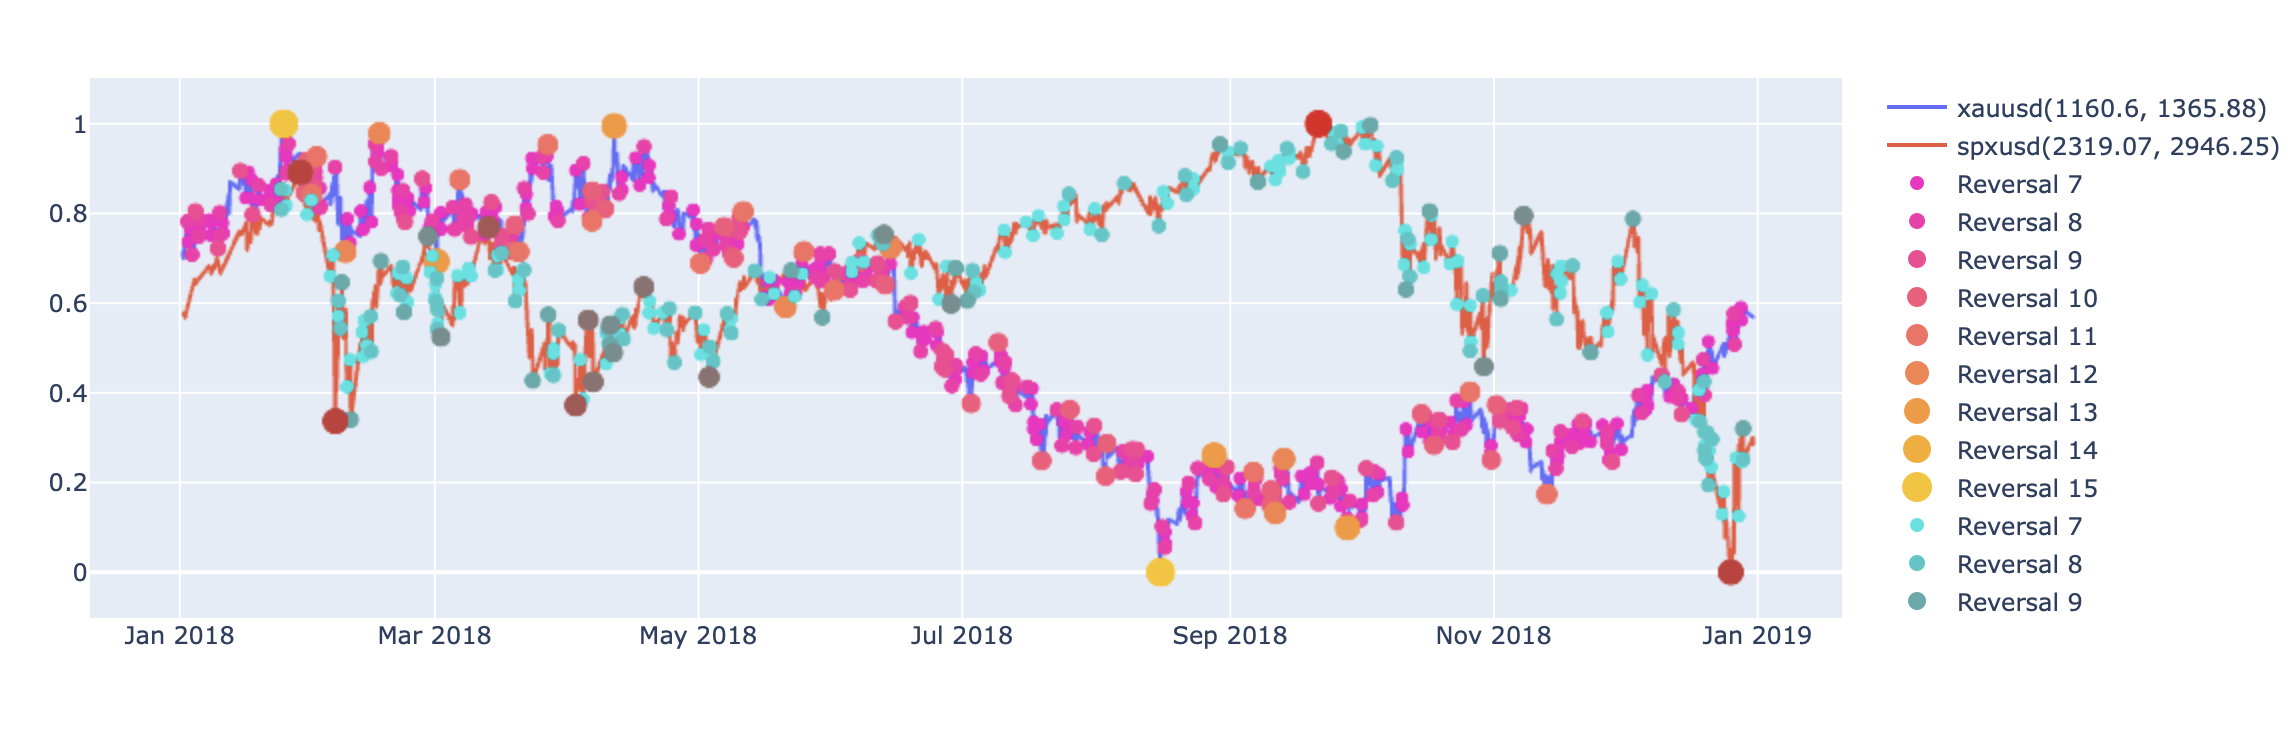
\includegraphics[width=1.05\textwidth]{Images/GoldSP500.png}
    \caption{Gold ounce in USD vs S$\&$P500 index  (scaled)}
    \label{fig:GoldSP500Scalled}
\end{figure}


\section{Extensions}
\subsection{The Pathogen algorithm}
The Pathogen algorithm \cite{Pathogen} uses the GraphX library to find causal inference between time related events. The idea behind this algorithm can be described with the following simplified example: $$\textit{the rooster crows immediately before the sunrise},$$ $$\textit{the rooster causes the sun to rise.}$$\\
Having isolated events, it converts them into a graph base model in order to look into the causal links between events. The causality measure is propagated through the graph until some convergence criteria is met. By extracting the attribute values for each element, the causal links will be found. \\
The algorithm is implemented on a library where the main two packages are the following:
\begin{itemize}
    \item \textbf{Rooster}: The Rooster takes as input some time related events structured as a resilient distributed data set (rdd) of events and generates a graph (GraphX) with vertices that contain specific attributes and edges with the weights of the causal links. Then, it observes a true causation signal on the events by generating random correlations (some noise) over the same events but on different times (uses Monte Carlo simulations to check if it is a true causal link or just a simple coincidence) and back propagating the scores to their most connected events.
    After that, each event will be linked to many other with specific weights. 
    Then, it outputs the causal effects found (the observed and normalised correlations) structured as a graph.
  
    \item \textbf{Sun}: The Sun takes as input the output of the Rooster and extracts the most probable causes and effects by returning a new graph where vertices contain the score of two measures. The latter are related with the likelihood of the event to cause or to be caused by other events:

    
    \begin{itemize}
        \item \textbf{Aggressiveness}: how likely an event could explain downstream effects.
        \item \textbf{Sensitivity}: how likely an event results from an upstream event cause.
    \end{itemize}
    \end{itemize}

%\subsubsection{Modifications}
%Several unit tests have been performed on Pathogen, as well as some upgrades to be compatible to newer versions of Scala and Spark (Scala $2.12$ and Spark $3.1.2$).


\subsubsection{Connection with TrendCalculus}
Pathogen is utilised aiming to establish causal inference on bi-variate time series. The main goal behind using this algorithm is to create a causal network in which the time series are converted to events that are then turned into graphs. These graphs are then to be analysed and hopefully provide meaningful insight. \\[2ex]
Since the output of TrendCalculus is a time series of trend change points (reversal points) and the input of Pathogen is a set of events, it is necessary to transform the one into the other. 
Therefore, an event in this case is designed to be the occurrence of consecutive reversal points for a specific reversal order. Each event carries information regarding the dated reversals of the time series and the intervals that rise from them. 
For each of these intervals, the next information has been extracted and passed to the corresponding event:
\begin{itemize}
    \item Concept Id: identifier of the events. This number describes the specific reversal order considered, the time series the event belongs to, the positive or negative behaviour of the trend and the weight assigned to the event's slope. 
        %\vspace{0.1in}
           \begin{figure}[!ht]
           \centering
           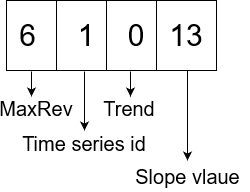
\includegraphics[scale=0.5]{Images/id.png}
           \caption{Example of the encoding of an event's Id}
           \label{fig:id}
       \end{figure}
        The concept id shown in Figure \ref{fig:id} corresponds to an event from the time series with concept id $1$ (Oil), reversal order of $6$, falling trend and the slope weight is $13$. 
    \item Start/End time of the event.
    \item Start/End value of the event. 
    \item Trend: if the trend is rising, the event will have trend value equal to $1$ and if it is falling, it will have trend equal to $0$.
    \item Width: the width of the interval, i.e the duration of the event.  
    \item MaxRev: the specific reversal order considered in each case.
    \item Slope: slope value of the rising or falling trends. 
    \item Normalised Slope: once the slope is obtained, it is normalised so it can take a number between 0 and 20 indicating the slope weight. 
    \item Amplitude: a value between $0$ and $1$. It is computed by measuring the distances between one event from one time series and the events from the other time series. If the event does not overlap with any of the events in the other time series and the distance between the closest one is very large, its amplitude will be 0. But if the events overlap with any, its amplitude will be $1$. In any other case, the amplitude will be equal to $e^{-d}$.
\end{itemize}
After several processing steps, the extracted information from the TrendCalculus time series is shown on Figure \ref{fig:data}.
\begin{figure}[!ht]
    \begin{BVerbatim}[baselinestretch=0.1,fontsize=\fontsize{6.8}{0}\selectfont]
   
+---------+--------------+------------+-------------------+-------------------+-----+------+------+------+---------------+---------+
|conceptId|start_of_event|end_of_event|        start_value|          end_value|trend| width|maxRev| slope|normalisedSlope|amplitude|
+---------+--------------+------------+-------------------+-------------------+-----+------+------+------+---------------+---------+
|    61013|    1325586960|  1325590140|0.40563991323210513|0.15618221258134468|    0|  3180|     6|-0.685|             13|    0.272|
|     6111|    1325590140|  1325647080|0.15618221258134468| 0.6203904555314533|    1| 56940|     6| 0.067|              1|      1.0|
|     6103|    1325647080|  1325660460| 0.6203904555314533| 0.3535791757049882|    0| 13380|     6|-0.177|              3|      1.0|
|     6110|    1325660460|  1325761980| 0.3535791757049882| 0.6442516268980476|    1|101520|     6| 0.021|              0|      1.0|
|     6116|    1325761980|  1325770920| 0.6442516268980476|                1.0|    1|  8940|     6| 0.341|              6|      1.0|
+---------+--------------+------------+-------------------+-------------------+-----+------+------+------+---------------+---------+
\end{BVerbatim}
    \caption{All of the extracted information from the TrendCalculus times series.}
    \label{fig:data}
\end{figure}
\\Once the data has been extracted from the financial time series, we keep only the necessary columns for Pathogen (Figure \ref{fig:data_pathogen}): concept id, start of the event, end of the event and amplitude.
\begin{figure}[!ht]
\centering
    \begin{BVerbatim}[baselinestretch=0.1,fontsize=\fontsize{12}{0}\selectfont]
+---------+----------+----------+---------+
|conceptId|eventStart| eventStop|amplitude|
+---------+----------+----------+---------+
|    61013|1325586960|1325590140|    0.272|
|     6111|1325590140|1325647080|      1.0|
|     6103|1325647080|1325660460|      1.0|
|     6110|1325660460|1325761980|      1.0|
|     6116|1325761980|1325770920|      1.0|
+---------+----------+----------+---------+
    \end{BVerbatim}
    \caption{Example of a set of events - input to Pathogen}
    \label{fig:data_pathogen}
\end{figure}


\subsection{Experiments}
One major issue that occurred during the stacking of the two algorithms is that different reversal orders of the two time series came with significantly different interval widths of consecutive reversals. To handle this issue and choose the optimal pair of orders, we used the Kolmogorov-Smirnov statistic. Specifically, the optimal pair was chosen as the one with the smallest Kolmogorov-Smirnov statistic between the empirical distribution functions of the time widths between consecutive reversals. The results of these experiments are summarised by the value of the Kolmogorov-Smirnov statistic on tables \ref{table:gold_oil}, \ref{table:gold_s&p500}. Notably, the optimal values for the reversal orders for Gold and Oil turn out to be $7$ and $6$ respectively; a result that was expected after visual inspection of the graph of Figure \ref{fig:GoldOilScalled}. For the Gold price and the S$\&$P$500$ index, the respective pair of orders turns out to be again $7$ and $6$. 

\vspace{0.3in}
\begin{table}[h!]
\centering
\begin{tabular}{|
>{\columncolor[HTML]{9E1A1A}}c |
>{\columncolor[HTML]{FEDAD7}}c |
>{\columncolor[HTML]{FEDAD7}}c |
>{\columncolor[HTML]{FEDAD7}}c |
>{\columncolor[HTML]{FEDAD7}}c |
>{\columncolor[HTML]{FEDAD7}}c |
>{\columncolor[HTML]{FEDAD7}}c |
>{\columncolor[HTML]{FEDAD7}}c |
>{\columncolor[HTML]{FEDAD7}}c |
>{\columncolor[HTML]{FEDAD7}}c |
>{\columncolor[HTML]{FEDAD7}}c |}
\hline
{\color[HTML]{FFFFFF} Reversal order} & \cellcolor[HTML]{9E1A1A}{\color[HTML]{FFFFFF} 6} & \cellcolor[HTML]{9E1A1A}{\color[HTML]{FFFFFF} 7} & \cellcolor[HTML]{9E1A1A}{\color[HTML]{FFFFFF} 8} & \cellcolor[HTML]{9E1A1A}{\color[HTML]{FFFFFF} 9} & \cellcolor[HTML]{9E1A1A}{\color[HTML]{FFFFFF} 10} & \cellcolor[HTML]{9E1A1A}{\color[HTML]{FFFFFF} 11} & \cellcolor[HTML]{9E1A1A}{\color[HTML]{FFFFFF} 12} & \cellcolor[HTML]{9E1A1A}{\color[HTML]{FFFFFF} 13} & \cellcolor[HTML]{9E1A1A}{\color[HTML]{FFFFFF} 14} & \cellcolor[HTML]{9E1A1A}{\color[HTML]{FFFFFF} 15} \\ \hline
{\color[HTML]{FFFFFF} 6}              & 0.16                                             & 0.39                                             & 0.6                                              & 0.73                                             & 0.83                                              & 0.94                                              & 1.0                                               & 1.0                                               & 1.0                                               & 1.0                                               \\ \hline
{\color[HTML]{FFFFFF} 7}              & \textbf{0.05}                                    & 0.19                                             & 0.40                                             & 0.59                                             & 0.74                                              & 0.90                                              & 1.0                                               & 0.99                                              & 1.0                                               & 1.0                                               \\ \hline
{\color[HTML]{FFFFFF} 8}              & 0.25                                             & 0.47                                             & 0.22                                             & 0.40                                             & 0.63                                              & 0.82                                              & 0.99                                              & 0.92                                              & {\color[HTML]{000000} 1.0}                        & 1.0                                               \\ \hline
{\color[HTML]{FFFFFF} 9}              & 0.40                                             & 0.2                                              & 0.06                                             & 0.24                                             & 0.46                                              & 0.67                                              & 0.88                                              & 0.91                                              & 1.0                                               & 1.0                                               \\ \hline
{\color[HTML]{FFFFFF} 10}             & 0.60                                             & 0.42                                             & 0.22                                             & 0.47                                             & 0.28                                              & 0.5                                               & 0.7                                               & 0.8                                               & 0.99                                              & 0.99                                              \\ \hline
{\color[HTML]{FFFFFF} 11}             & 0.74                                             & 0.61                                             & 0.43                                             & 0.2                                              & 0.08                                              & 0.3                                               & 0.5                                               & 0.7                                               & 0.93                                              & 0.88                                              \\ \hline
{\color[HTML]{FFFFFF} 12}             & 0.92                                             & 0.8                                              & 0.64                                             & 0.42                                             & 0.22                                              & 0.09                                              & 0.42                                              & 0.54                                              & 0.73                                              & 0.67                                              \\ \hline
{\color[HTML]{FFFFFF} 13}             & 0.97                                             & 0.9                                              & 0.75                                             & 0.64                                             & 0.47                                              & 0.26                                              & 0.25                                              & 0.37                                              & 0.57                                              & 0.48                                              \\ \hline
{\color[HTML]{FFFFFF} 14}             & 0.92                                             & 0.92                                             & 0.9                                              & 0.8                                              & 0.65                                              & 0.45                                              & 0.31                                              & 0.27                                              & 0.5                                               & 0.43                                              \\ \hline
{\color[HTML]{FFFFFF} 15}             & 1.0                                              & 1.0                                              & 1.0                                              & 1.0                                              & 0.98                                              & 0.8                                               & 0.53                                              & 0.57                                              & 0.35                                              & 0.47                                              \\ \hline
\end{tabular}
\caption{Gold/Oil}
\label{table:gold_oil}
\end{table}




% Please add the following required packages to your document preamble:
% \usepackage[table,xcdraw]{xcolor}
% If you use beamer only pass "xcolor=table" option, i.e. \documentclass[xcolor=table]{beamer}
\begin{table}[h!]
\centering
\begin{tabular}{|
>{\columncolor[HTML]{9E1A1A}}c |
>{\columncolor[HTML]{FEDAD7}}c |
>{\columncolor[HTML]{FEDAD7}}c |
>{\columncolor[HTML]{FEDAD7}}c |
>{\columncolor[HTML]{FEDAD7}}c |
>{\columncolor[HTML]{FEDAD7}}c |
>{\columncolor[HTML]{FEDAD7}}c |
>{\columncolor[HTML]{FEDAD7}}c |
>{\columncolor[HTML]{FEDAD7}}c |}
\hline
{\color[HTML]{FFFFFF} \textbf{Reversal order}} & \cellcolor[HTML]{9E1A1A}{\color[HTML]{FFFFFF} \textbf{6}} & \cellcolor[HTML]{9E1A1A}{\color[HTML]{FFFFFF} \textbf{7}} & \cellcolor[HTML]{9E1A1A}{\color[HTML]{FFFFFF} \textbf{8}} & \cellcolor[HTML]{9E1A1A}{\color[HTML]{FFFFFF} \textbf{9}} & \cellcolor[HTML]{9E1A1A}{\color[HTML]{FFFFFF} \textbf{10}} & \cellcolor[HTML]{9E1A1A}{\color[HTML]{FFFFFF} \textbf{11}} & \cellcolor[HTML]{9E1A1A}{\color[HTML]{FFFFFF} \textbf{12}} & \cellcolor[HTML]{9E1A1A}{\color[HTML]{FFFFFF} \textbf{13}} \\ \hline
{\color[HTML]{FFFFFF} \textbf{6}}              & 0.25                                                      & 0.47                                                      & 0.65                                                      & 0.75                                                      & 0.88                                                       & 0.96                                                       & 1.0                                                        & 1.0                                                        \\ \hline
{\color[HTML]{FFFFFF} \textbf{7}}              & \textbf{0.05}                                             & 0.27                                                      & 0.46                                                      & 0.64                                                      & 0.81                                                       & 0.93                                                       & 1.0                                                        & 1.0                                                        \\ \hline
{\color[HTML]{FFFFFF} \textbf{8}}              & 0.16                                                      & 0.09                                                      & 0.3                                                       & 0.48                                                      & 0.7                                                        & 0.9                                                        & 0.97                                                       & 0.96                                                       \\ \hline
{\color[HTML]{FFFFFF} \textbf{9}}              & 0.32                                                      & 0.11                                                      & 0.13                                                      & 0.3                                                       & 0.55                                                       & 0.76                                                       & 0.83                                                       & 0.8                                                        \\ \hline
{\color[HTML]{FFFFFF} \textbf{10}}             & 0.53                                                      & 0.31                                                      & 0.14                                                      & 0.14                                                      & 0.4                                                        & 0.59                                                       & 0.74                                                       & 0.67                                                       \\ \hline
{\color[HTML]{FFFFFF} \textbf{11}}             & 0.67                                                      & 0.51                                                      & 0.32                                                      & 0.13                                                      & 0.23                                                       & 0.4                                                        & 0.66                                                       & 0.67                                                       \\ \hline
{\color[HTML]{FFFFFF} \textbf{12}}             & 0.87                                                      & 0.7                                                       & 0.55                                                      & 0.34                                                      & 0.12                                                       & 0.24                                                       & 0.6                                                        & 0.67                                                       \\ \hline
{\color[HTML]{FFFFFF} \textbf{13}}             & 0.95                                                      & 0.8                                                       & 0.7                                                       & 0.55                                                      & 0.35                                                       & 0.16                                                       & 0.41                                                       & 0.6                                                        \\ \hline
{\color[HTML]{FFFFFF} \textbf{14}}             & 0.93                                                      & 0.91                                                      & 0.84                                                      & 0.73                                                      & 0.53                                                       & 0.34                                                       & 0.34                                                       & 0.38                                                       \\ \hline
{\color[HTML]{FFFFFF} \textbf{15}}             & 1.0                                                       & 1.0                                                       & 1.0                                                       & 1.0                                                       & 0.92                                                       & 0.7                                                        & 0.37                                                       & 0.34                                                       \\ \hline
\end{tabular}
\caption{Gold/S\&P500}
\label{table:gold_s&p500}
\end{table}
\section{Results and Interpretation}
The full sets of events over the last two decades from the two time series (with the structure shown in Figure \ref{fig:data_pathogen}) are merged together into a single set of events and it is passed as input to Pathogen. After calling the Rooster and the Sun methods, the information of interest lays on the edges and vertices of the returned graph. For interpretation purposes the vertices are joined together while including the normalised correlation among them and their corresponding causal measures (Figure \ref{fig:graph}).
\begin{figure}[!ht]
\centering
    \begin{BVerbatim}[baselinestretch=0.1,fontsize=\fontsize{12}{0}\selectfont]
+-----+-----+--------+--------------+-----------+
|  src|  dst|normCorr|aggressiveness|sensitivity|
+-----+-----+--------+--------------+-----------+
| 7212| 6117|     1.0|       0.01239|    0.00466|
| 7210|61014| 0.92592|       0.14875|    0.01913|
| 7210|61113| 0.80645|       0.14875|    0.01669|
| 7200|61120| 0.70422|       0.11715|    0.01017|
| 6110|72010| 0.63291|       0.11295|    0.02130|
| 7200|61017|     0.6|       0.11715|    0.01743|
| 7210|61111| 0.56818|       0.14875|    0.00863|
| 6111|61017|     0.5|       0.01809|    0.01743|
|61017| 6111|     0.5|       0.01731|    0.01821|
| 7204|61012|     0.5|       0.02667|    0.01613|
+-----+-----+--------+--------------+-----------+
    \end{BVerbatim}
    \caption{Example - Output of Pathogen: The \textit{src} and \textit{dst} indicate the event id's of the related vertices, the \textit{normCorr} stands for the normalised correlation and the last two arguments are the returned causality measures.}
    \label{fig:graph}
\end{figure}
\\The first row of the table in Figure \ref{fig:graph},  can be interpreted as follows: the event $7212$, i.e., encoding reversal order $7$ of gold price $(2)$ rising $(1)$ by normalised slope $2$ between $(2/20$ and $3/20)$ and event $6117$, i.e., encoding reversal order $6$ of oil price $(1)$ rising $(1)$ by normalised slope $7$ between $(7/20$ and $8/20)$, have the highest normalised correlation of $1.0$ but with limited aggressiveness $0.01239$ and sensitivity $0.00466$. Meaning that, \textit{a slight rise in the gold price of reversal order $7$ precedes a medium rise in oil price of reversal order $6$.}\\[3ex]
% \begin{figure}[ht!]
% \centering
%     \begin{BVerbatim}[baselinestretch=0.1,fontsize=\fontsize{12}{0}\selectfont]
% +-----+-----+------------------+--------------------+--------------------+
% |  src|  dst|          normCorr|      aggressiveness|         sensitivity|
% +-----+-----+------------------+--------------------+--------------------+
% | 7212| 6117|               1.0|0.012391763797138798| 0.00465969871699266|
% +-----+-----+------------------+--------------------+--------------------+
%     \end{BVerbatim}
%     \caption{Row 1 - Output of Pathogen}
%     \label{fig:graph1}
% \end{figure}
Focusing on the second and third row, isolated on the table of Figure \ref{fig:graph2} one can see that, 
the event $7210$, i.e., a small rise in gold price at order $7$, seems to precede both $61014$ and $61113$, which are order $6$ oil price fall and rise of fairly steep normalised slopes. In other words, there is strong evidence for \textit{a slight rise in gold price seeming to just precede a rather sharp fall or rise in the oil price} at orders 6 and 7, respectively.
\begin{figure}[!h]
\centering
    \begin{BVerbatim}[baselinestretch=0.1,fontsize=\fontsize{12}{0}\selectfont]
+-----+-----+--------+--------------+-----------+
|  src|  dst|normCorr|aggressiveness|sensitivity|
+-----+-----+--------+--------------+-----------+
| 7210|61014| 0.92592|       0.14875|    0.01913|
| 7210|61113| 0.80645|       0.14875|    0.01669|
+-----+-----+--------+--------------+-----------+
    \end{BVerbatim}
    \caption{Rows 2 and 3 - Output of Pathogen}
    \label{fig:graph2}
\end{figure}
\\Another set of pairs that is worth noticing is shown on the table of Figure \ref{fig:graph3}.
\begin{figure}[!ht]
\centering
    \begin{BVerbatim}[baselinestretch=0.1,fontsize=\fontsize{12}{0}\selectfont]
+-----+-----+--------+--------------+-----------+
|  src|  dst|normCorr|aggressiveness|sensitivity|
+-----+-----+--------+--------------+-----------+
| 7200|61120| 0.70422|       0.11715|    0.01017|
| 7200|61017|     0.6|       0.11715|    0.01743|
+-----+-----+--------+--------------+-----------+
    \end{BVerbatim}
    \caption{Rows 4 and 6 - Output of Pathogen}
    \label{fig:graph3}
\end{figure}
Looking at these two pairs of events and their associated causal measures, they seem to suggest that when the order $7$ gold price begins to fall with the smallest normalised slope in (0,1/20), corresponding to event $7200$, the order $6$ in oil price begins to rise and fall sharply by the greatest normalised slopes in (17/20, 20/20). \textit{This seems to indicate that a drop in gold price seems to precede a sharp rise and fall in oil price.}\\[2ex]
Yet another interesting pair of events seen in Figure \ref{fig:graph4}, suggests that a small rise in order $6$ oil price (event $6110$) precedes an order $7$ gold price decrease with a moderately large normalised (negative) slope in ($10/20$,$11/20$).
\begin{figure}[!ht]
\centering
    \begin{BVerbatim}[baselinestretch=0.1,fontsize=\fontsize{12}{0}\selectfont]
+-----+-----+--------+--------------+-----------+
|  src|  dst|normCorr|aggressiveness|sensitivity|
+-----+-----+--------+--------------+-----------+
| 6110|72010| 0.63291|       0.11295|    0.02130|
+-----+-----+--------+--------------+-----------+
    \end{BVerbatim}
    \caption{Row 5 - Output of Pathogen}
    \label{fig:graph4}
\end{figure}
\\This seems to suggest that there may be other time series one may want to consider such as the S$\&$P$500$ index, tech stocks, etc., as the drop in gold price may be due to other factors in markets and media apart from the influence of oil price. Thankfully, the framework here can scale to hundreds of time series (not just two).\\[2ex]
All of the above interpretations should be made with a grain of salt and only seen as a first step towards scalable causal inference. Lastly, Figure \ref{fig:graph5} shows the result when it orders the most aggressive \textit{src} events affecting \textit{dst} events so we can get a better idea of the most effective \textit{src} events.
\begin{figure}[!ht]
\centering
    \begin{BVerbatim}[baselinestretch=0.1,fontsize=\fontsize{12}{0}\selectfont]
+----+-----+--------+--------------+-----------+
| src|  dst|normCorr|aggressiveness|sensitivity|
+----+-----+--------+--------------+-----------+
|7210| 6116| 0.10608|       0.14875|    0.00485|
|7210| 7209| 0.13089|       0.14875|    0.00814|
|7210| 7213| 0.12626|       0.14875|    0.00996|
|7210| 6108| 0.16199|       0.14875|    0.00975|
|7210| 6111| 0.14051|       0.14875|    0.01821|
+----+-----+--------+--------------+-----------+
    \end{BVerbatim}
    \caption{Example - Output of Pathogen ordered by descending aggressiveness value}
    \label{fig:graph5}
\end{figure}

\section{Discussion and Conclusion}
The TrendCalculus algorithm provides a powerful solution on identifying major trend change points and is complemented with an interactive visualisation tool that allows the user to focus on any time window of interest. The latter, is quite sufficient on illustrating more than one reversal time series which can be beneficial for comparison purposes. This way, the user can gain some intuition from visual inspection on bi-variate time series. Then, the outcome can be used as input to Pathogen in an attempt to find causal inference on time related events. Notably, the implementation is not limited to financial time series, but rather can receive as input any time series. In addition, Pathogen seems to capture part of our intuition regarding the co-movement of Gold and Oil prices but also suggests that other factors should be put under question. We believe that the combination of the two algorithms that have the distinguishing feature of being able to scale to arbitrarily large data sets can be very beneficial for discovering causal inference among multivariate time series.

% Final deep dive on the getEventsCorrelation method :
% The correlations found are indeed the sum of amplitudes. However, not the amplitudes of the original events!
% The getTicks method creates additional events based on the last time (nextTime in Pathogen) found before the endTime. The way this is done is by iterating like this:
% nextTime = startTime
% while nextTime.isBefore(endTime)
% nextTime = nextTime.plusMinute(1)
% Then the events are returned with an additional column of nextTime. After that the different events are joined on an Array with elements(event i, event j). The joined condition is the nextTime. Lastly, the elements are joined  by key. On every pair of joined events the correlation is found by summing the amplitudes. Eg: events 2 and 5 have correlation 6.0 . If we look at the events returned by the getTicks method we see the following

% NextTime value for the events with conceptId 5 and 2:
% 5: 1609740000 1609800000 1609860000
% 2: 1609740000 1609800000 1609860000

% Then the pair (2-5) appears three times inside the events correlation. So I assume that the join condition is the NextTime.

% One thing is that I transformed the times from unix to timestamp to see if the result makes sense. Unfortunately it doesnt. My speculation is that this is because we are using 3 different types: seconds, minutes and milliseconds. This is problematic because the condition: nextTime.isBefore(endTime) sometimes is met but looking at the timestamps it is wrong.

% I am not sure how looking at the last minute before the end of the event and joining events together if they end at the same time can be meaningfully interpreted. However, I hope this makes things a bit more clear when it comes to understanding the correlation



\section{Future and Current Work}
In order to perform a more thorough interpretation of the results, the graph resulted from Pathogen can be transformed into Fuzzy cognitive maps: causal relations. 
Our current project work is available as examples and notebooks at \cite{TrendCalculusNotebooks} and \cite{PathogenNotebooks}. 


\section{Acknowledgements}

This project was supported by {\em Combient Mix AB} through a {\em Data Science Project Fellowships} between 2021-10 and 2021-12 to Stavroula Rafailia Vlachou and Virginia Jimenez Mohedano at {\em Combient Competence Centre for Data Engineering Sciences}, Department of Mathematics, Uppsala University, Uppsala, Sweden, and {\em Databricks University Alliance} with infrastructure credits from {\em AWS} to Raazesh Sainudiin, Department of Mathematics, Uppsala University, Sweden. Many thanks to Andrew Morgan and Antoine Amend for their guidance.

\nocite{*}
\printbibliography

\end{document}